% TODO: Decide on paper figures!!

%%%%%%%%%%%%%%%%%%%%%%%%%%%%%%%%%%%%%%%%%%%%%%%%%%%%%%%%%%%%%%%%%%%%%%%%%%%%%%

\documentclass[review,journal]{vgtc}
\usepackage{microtype}
\usepackage{clrscode}
\usepackage{mathptmx}
\usepackage{graphicx}
\usepackage{times}
\usepackage{xspace}
\onlineid{277}
\vgtccategory{Research}
\vgtcinsertpkg

\newcommand{\Shade}{\texttt{Shade}\xspace}
\title{Lux: Composable, High-Performance Visualization for the Web}
\author{Carlos Scheidegger}
\authorfooter{\item Carlos Scheidegger is with AT\&T Research, email: cscheid@research.att.com}
\shortauthortitle{Scheidegger: Lux}

\abstract{
We address the problem of writing succinct and expressive programs for
high-performance, interactive visualizations on the web.
%
Modern web browsers provide WebGL, which exposes hardware-accelerated
graphics and enables high-performance graphics on the web.
%
In this paper, we consider the WebGL API in the context of creating reusable
building blocks, and identify some key shortcomings. We present
Lux, designed explicitly to address these shortcomings.
%
Lux is a \emph{domain-specific embedded language}, built around an
optimizing source-to-source compiler.
%
Among other advantages, it gives users access to GPU programming without
requiring them to write GLSL, the C-like vertex and fragment
shading languages embedded in WebGL. Lux is capable of
automatically \emph{deriving shaders}, reducing needless
repetition and increasing source code reuse.
%
We provide experimental evidence of Lux's ability to provide
higher-level abstractions than previously possible, with a fraction of
the effort necessary with currently-available libraries.
}

\keywords{DSEL, WebGL, visualization toolkits}

\teaser{
\centering

\includegraphics[width=\linewidth]{fig/teaser/teaser.png}
\caption{LOOK AT MY AWESOME TEASER. JUST LOOK AT IT}
}

\begin{document}

\firstsection{Introduction}

\maketitle

Modern web browsers now expose much of the hardware-accelerated
graphics API and computing power that only a few decades ago were
exclusive of supercomputers.
%
Together with the ubiquity of graphics
cards in the desktop and the rise of the world-wide web as a platform
for application development and deployment, visualization researchers
now have a clear opportunity to move high-performance visualizations to
the world-wide web.
%
The current state-of-the-art API for three-dimensional web-based
graphics is WebGL~\cite{webgl-spec}, an open standard based on OpenGL
ES 2.0~\cite{opengles-spec} (here, ES stands for ``Embedded
Systems'').

WebGL is a good API for exposing GPU capabilities,
but it is far from an ideal language for \emph{programming}.
%
It is based on a state machine, and exposes much of its functionality
via its vertex and fragment program languages. These languages allow
for powerful, high-performance computations, but they have
their own syntax and semantics separate from the host language (in
this case, Javascript). Therein lies a major problem:
WebGL libraries and applications written in pure Javascript 
suffer from ``impedance mismatch''.

In this paper, we contribute Lux, which seeks to remove one barrier
for the wider adoption of WebGL as an effective programming library
for high-performance graphics and visualization on the Web.
%
% FIXME This sentence belongs elsewhere
%
Lux was designed for WebGL, but the concepts generalize to
other high-level graphics APIs such as OpenGL 4 and Direct3D 11, and
other modern host languages such as C++, Java and Python.

The observations leading to Lux and the design decisions behind the
library are discussed in Section~\ref{sec:design}, after
Section~\ref{sec:relatedwork} reviews the relevant literature and
previous work and
places it in context of Lux's features. In
Section~\ref{sec:evaluation}, we provide evidence that Lux scales
well both in programming effort and in program performance. 
We finish the paper with Section~\ref{sec:discussion}, a discussion of
the implications of the presented work.

\section{Related Work\label{sec:relatedwork}}

\begin{figure*}
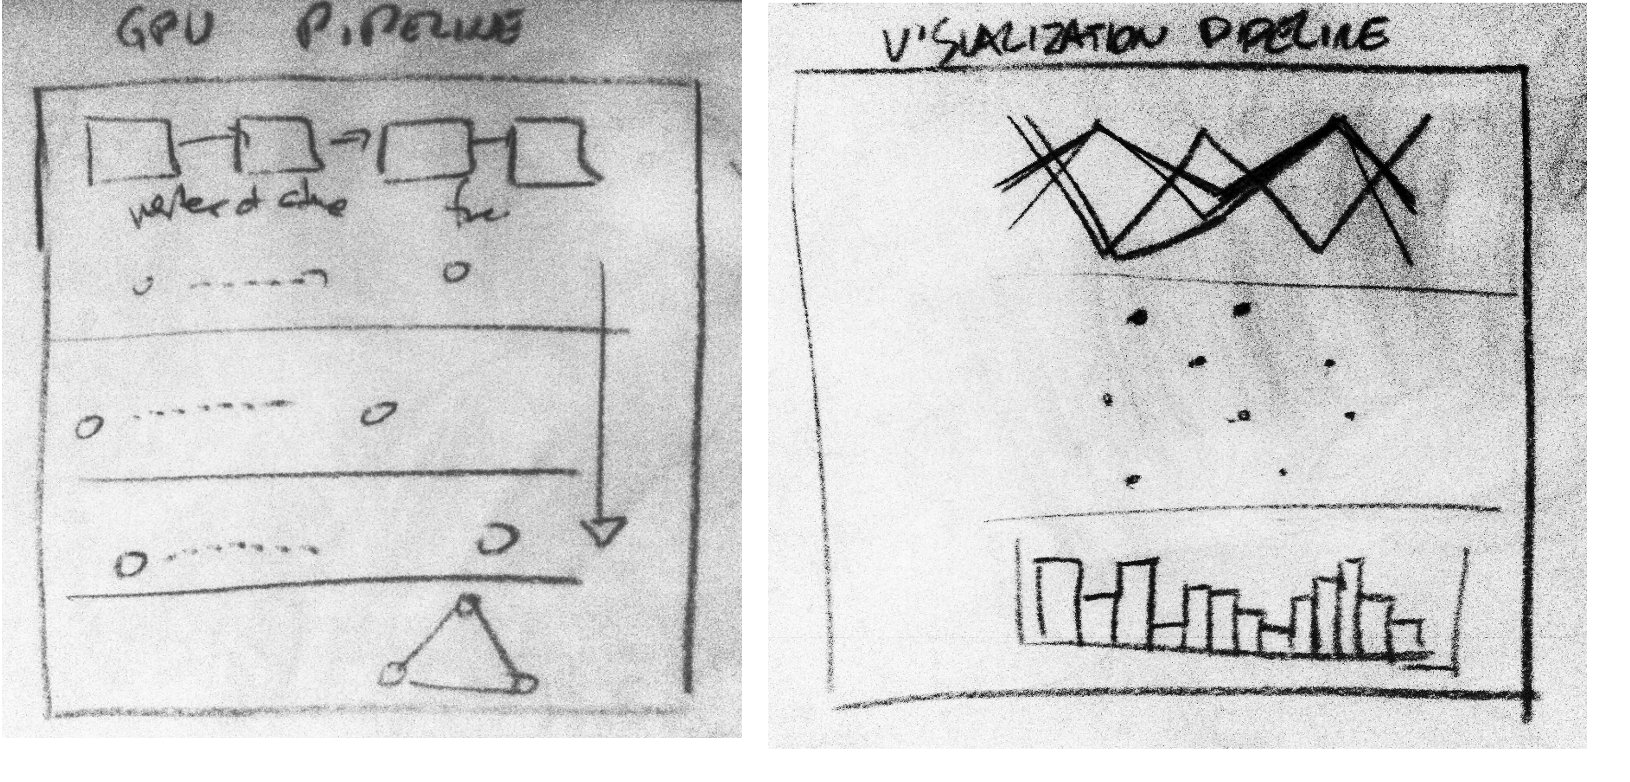
\includegraphics[width=\linewidth]{fig/pipeline_mismatch/pipeline_mismatch.jpg}
\caption{The fundamental impedance mismatch between the GPU pipeline
and the visualization pipeline.\label{fig:mismatch}}
\end{figure*}

The World-Wide Web has recently emerged as the primary means of
exchanging hypertext documents. As computing power has increased,
traditional hypertext has become intertwined with rich media such as
video and interactive graphics. Naturally, visualization and 3D
graphics have recently received substantial attention.

% visualization for the Web
Heer and co-authors have done early work in the design of effective
visualization and graphics infrastructure for the Web, including Java
libraries such as Prefuse~\cite{Heer:2005:PAT} (and its followup
Flare, based on Adobe's Flash runtime~\cite{Adobe:2011:Flash}).
Processing~\cite{Reas:2007:PAP} is a particularly successful example
of a graphics and visualization library built on the Java platform.
%
Lux, in contrast, is based on WebGL, which does not require plugins
and is an open standard~\cite{webgl-spec}.
%
Resig~\cite{Resig:2010:PJ} has recently released Processing.JS, a
Javascript port of Processing.
%
Although very useful in practice, Processing.JS aims to recreate most
of the Processing programming language and environment, and so has
similar impedance mismatch problems when integrated with Javascript
code.  In addition, Lux has better performance characteristics, as
we argue in Section~\ref{sec:evaluation}.

More recently, Protovis~\cite{Bostock:2009:PAG} and
$\textrm{D}^3$~\cite{Bostock:2011:DDD} have been proposed as modern
embodiments of visualization libraries for the web.  Both libraries
follow the critical observation that visualization specifications
should be \emph{declarative}: instead of specifying how to draw
something, they should specify what is to be drawn. In other words,
\emph{values} are emphasized over \emph{procedures}.
%
Lux takes a similar
approach with its abstraction of the WebGL shading infrastructure.
% 
Protovis (and portions of $\textrm{D}^3$) use Scalable Vector Graphics
(SVG~\cite{svg-spec}) as their graphics target, and SVG is much closer
to the rest of the ecosystem of the modern web. In particular, it
contains a full Document Object Model (DOM~\cite{dom-spec}). This has
two main consequences.
%
The upside of having access to the DOM is that much of the programming
model and software infrastructure in Javascript carries over to SVG
representations: the infrastructure for graphics theming, interaction
and so on are provided by the web browser itself. This is a big
advantage.
%
The downside is that using SVG incurs a performance penalty that might
be severe in large scale situations, as we describe in
section~\ref{sec:evaluation}.
%
With respect to API design, having access to the DOM has another
positive consequence: the distance to be reached between SVG
programming and Javascript programming is smaller. For example,
interactive visualization can be created by directly attaching
event handlers to DOM elements (such as ``mouse click'',
``mouse move'', etc.)
%
As we argue in Section~\ref{sec:design}, with WebGL, this gap is 
wider.
% Visualization libraries for the Web
% Protovis, D3.

Iris Inventor~\cite{Strauss:1993:IIA} (which later became Open
Inventor) was arguably among the original attempts to allow
higher-level programming constructs in programs using OpenGL-like
APIs.
%
Iris Inventor was built on top of IRIS GL, a proprietary ancestor of
OpenGL from the late 1980s.
%
There are myriad similar libraries such as OpenSG, OpenSceneGraph, and
NVIDIA's SceniX.
%
This happens in the WebGL ecosystem as well, with examples such as
Three.JS, X3DOM, SceneJS~\cite{SceneJS}, glge, and
SpiderGL~\cite{DiBenedetto:2010:SAJ}.
%
While all these libraries provide a large set of useful drawing
primitives, composing appearance specifications remains challenging.
%
SceneJS does generate some shader code automatically to fit the scene
graph description. Still, custom shader generation in SceneJS is
performed by textual source code injection. This is not optimal for
several reasons, including that managing variable naming conflicts is
brittle, and some optimizations become impossible.
% 3D Graphics of the Web
% three.js 

The observation that shading languages need their own layer of
abstraction is not new. In fact, Cook's pioneering work in Shade
Trees~\cite{Cook:1984:ST} comes largely from that observation.
%
McCool et al. later describe Sh, a shader metaprogramming
library~\cite{McCool:2002:SM} which is an early example
of embedding shading expressions in the host language
(in their case, C++). 
%
Lux takes this model even further:
most of its API is defined around denoting shading expressions
as Javascript values. While Sh requires explicit assignment of
expressions to vertex and fragment shaders, Lux 
%
Lux, in constrast, by default defers these decisions to the
compiler. This increases reuse: for example,
shader expressions can be hoisted to and from fragment and vertex
programming stages as necessary.
%
Recently,
Hanrahan and Foley have proposed Spark~\cite{Foley:2011:SMC}, a shader
programming language which shares much of the modularity and
composability design goals of Lux. 
%
In sharp contrast with Lux,
Spark is its own language with custom syntax and semantics. 
%
As we argue, part of the appeal in Lux's design is that it bridges
the gap between host and target languages. % which is caused by this decision.
%
% http://graphics.stanford.edu/papers/spark/spark_preprint.pdf
%
One practical advantage of insisting in an embedded DSL design is the
natural synergy that can be achieved. DSELs can easily be extended by host
libraries: for example, Pellacini's automatic shader simplication
technique~\cite{Pellacini:2005:UCA} could be implemented as a Javascript
module for Lux.

% Shading abstractions:
% Shade trees
% Shader meta-programming
% applications when shading abstractions are available:
% shader level of detail (pellacini)

\section{Design\label{sec:design}}

In this section we present the main aspects of Lux's design. We
start by describing what we call the \emph{fundamental impedance
mismatch} between the computational building blocks of graphics APIs
and the natural way to describe visualization specifications. Then, we
show how Lux tackles this problem and describe the major aspects of
the library.

\subsection{Visualization pipeline vs. GPU pipeline\label{sec:mismatch}}

Visualization specifications are, by and large, created by prescribing
encodings of data elements into attributes of visual primitives. This
observation dates all the way back to Bertin's original
work~\cite{Bertin:1967:SOG}, and pervades all formal approaches to
visualization design~\cite{Wickham:2009:GEG,Wilkinson:2005:TGO}. These
visual primitives can range from the very simplest, like a single dot,
to not-as-simple, such as a boxplot, to arbitrarily complex, such as
a polyline per data element in the case of parallel coordinates. 

In addition, the encoding of each attribute changes substantially from
case to case. Consider the differences in the following examples.  In
the case of a grand tour~\cite{Asimov:1985:TGT}, the visual primitive
is a simple dot, but the position of the dot involves computing a
projection of all coordinates of the multidimensional data point
(we can think of each sample as a vector with $k$ coordinates) along
the projection axes. In the case of parallel coordinates, the visual
primitive itself is a more complicated polyline, while the position of
the endpoints is simple to compute. Unlike the grand tour, there is a one-to-one
correspondence between the position of an endpoint and a single
coordinate of the multidimensional data point.  Finally, take the case
of the traditional histogram. There, each visual primitive is a
relatively simple rectangle with four vertices. Determining the height
of the rectangle, however, involves a computation
over \emph{all} input points. As Figure~\ref{fig:mismatch}
illustrates, each visualization uses a different access pattern over
the data.

This heterogeneity in access patterns is very much at
odds with the natural way to specify graphics computations in graphics
APIs such as WebGL, OpenGL and Direct3D. Referring again to
Figure~\ref{fig:mismatch}, note that graphics APIs are modeled very
closely to the underlying hardware, where data processing is done
``vertex-in, vertex-out''. If we specify vertex color, position,
etc. in the most natural fashion, the attributes need to be passed to
GPU in a one-to-one correspondence with the vertices. In other words,
if a visual encoding requires an array of $n$ vertices, an array of
exactly $n$ Cartesian positions will be necessary, together with an
array of exactly $n$ colors, and so on. Now, compare the case of a
Grand Tour visualization to that of parallel coordinates. A single
frame of a Grand Tour rendering takes $n$ vertices, while a single
frame of rendering parallel coordinates takes $n.k$ vertices, $n.k$
colors, etc. So if done in a straightforward manner, different
visualizations require different preprocessing steps over the
data, \emph{before} sending the data to the graphics card. This is
unfortunate, and especially so in relatively slower languages like
Javascript: we are stalling the fast graphics system by having the
CPU touch every vertex at every frame.

Modern graphics cards, however, are \emph{programmable}. What this
means is that the position and color of points and lines can be
determined by the result of an actual program execution. This
execution happens entirely in the GPU, in parallel (the
position of a vertex is independent of the position of the next
vertex). GPUs are quite parallel: a mobile device
such as Apple's latest iPad has four graphics cores, and consumer
video cards for desktops now have around two hundred ALUs executing GPU programs in
parallel. To achieve fast graphics, then, the data must reside
entirely on the graphics card, and the appropriate GPU programs for each visual
primitive must be written. This is the fundamental problem
which Lux seeks to address: how can we create a Javascript
visualization library which must be based around producing
GPU programs, while minimizing exposure to the quirks of the
underlying GPU programming model?

\subsection{From GLSL to Lux}

\begin{figure}
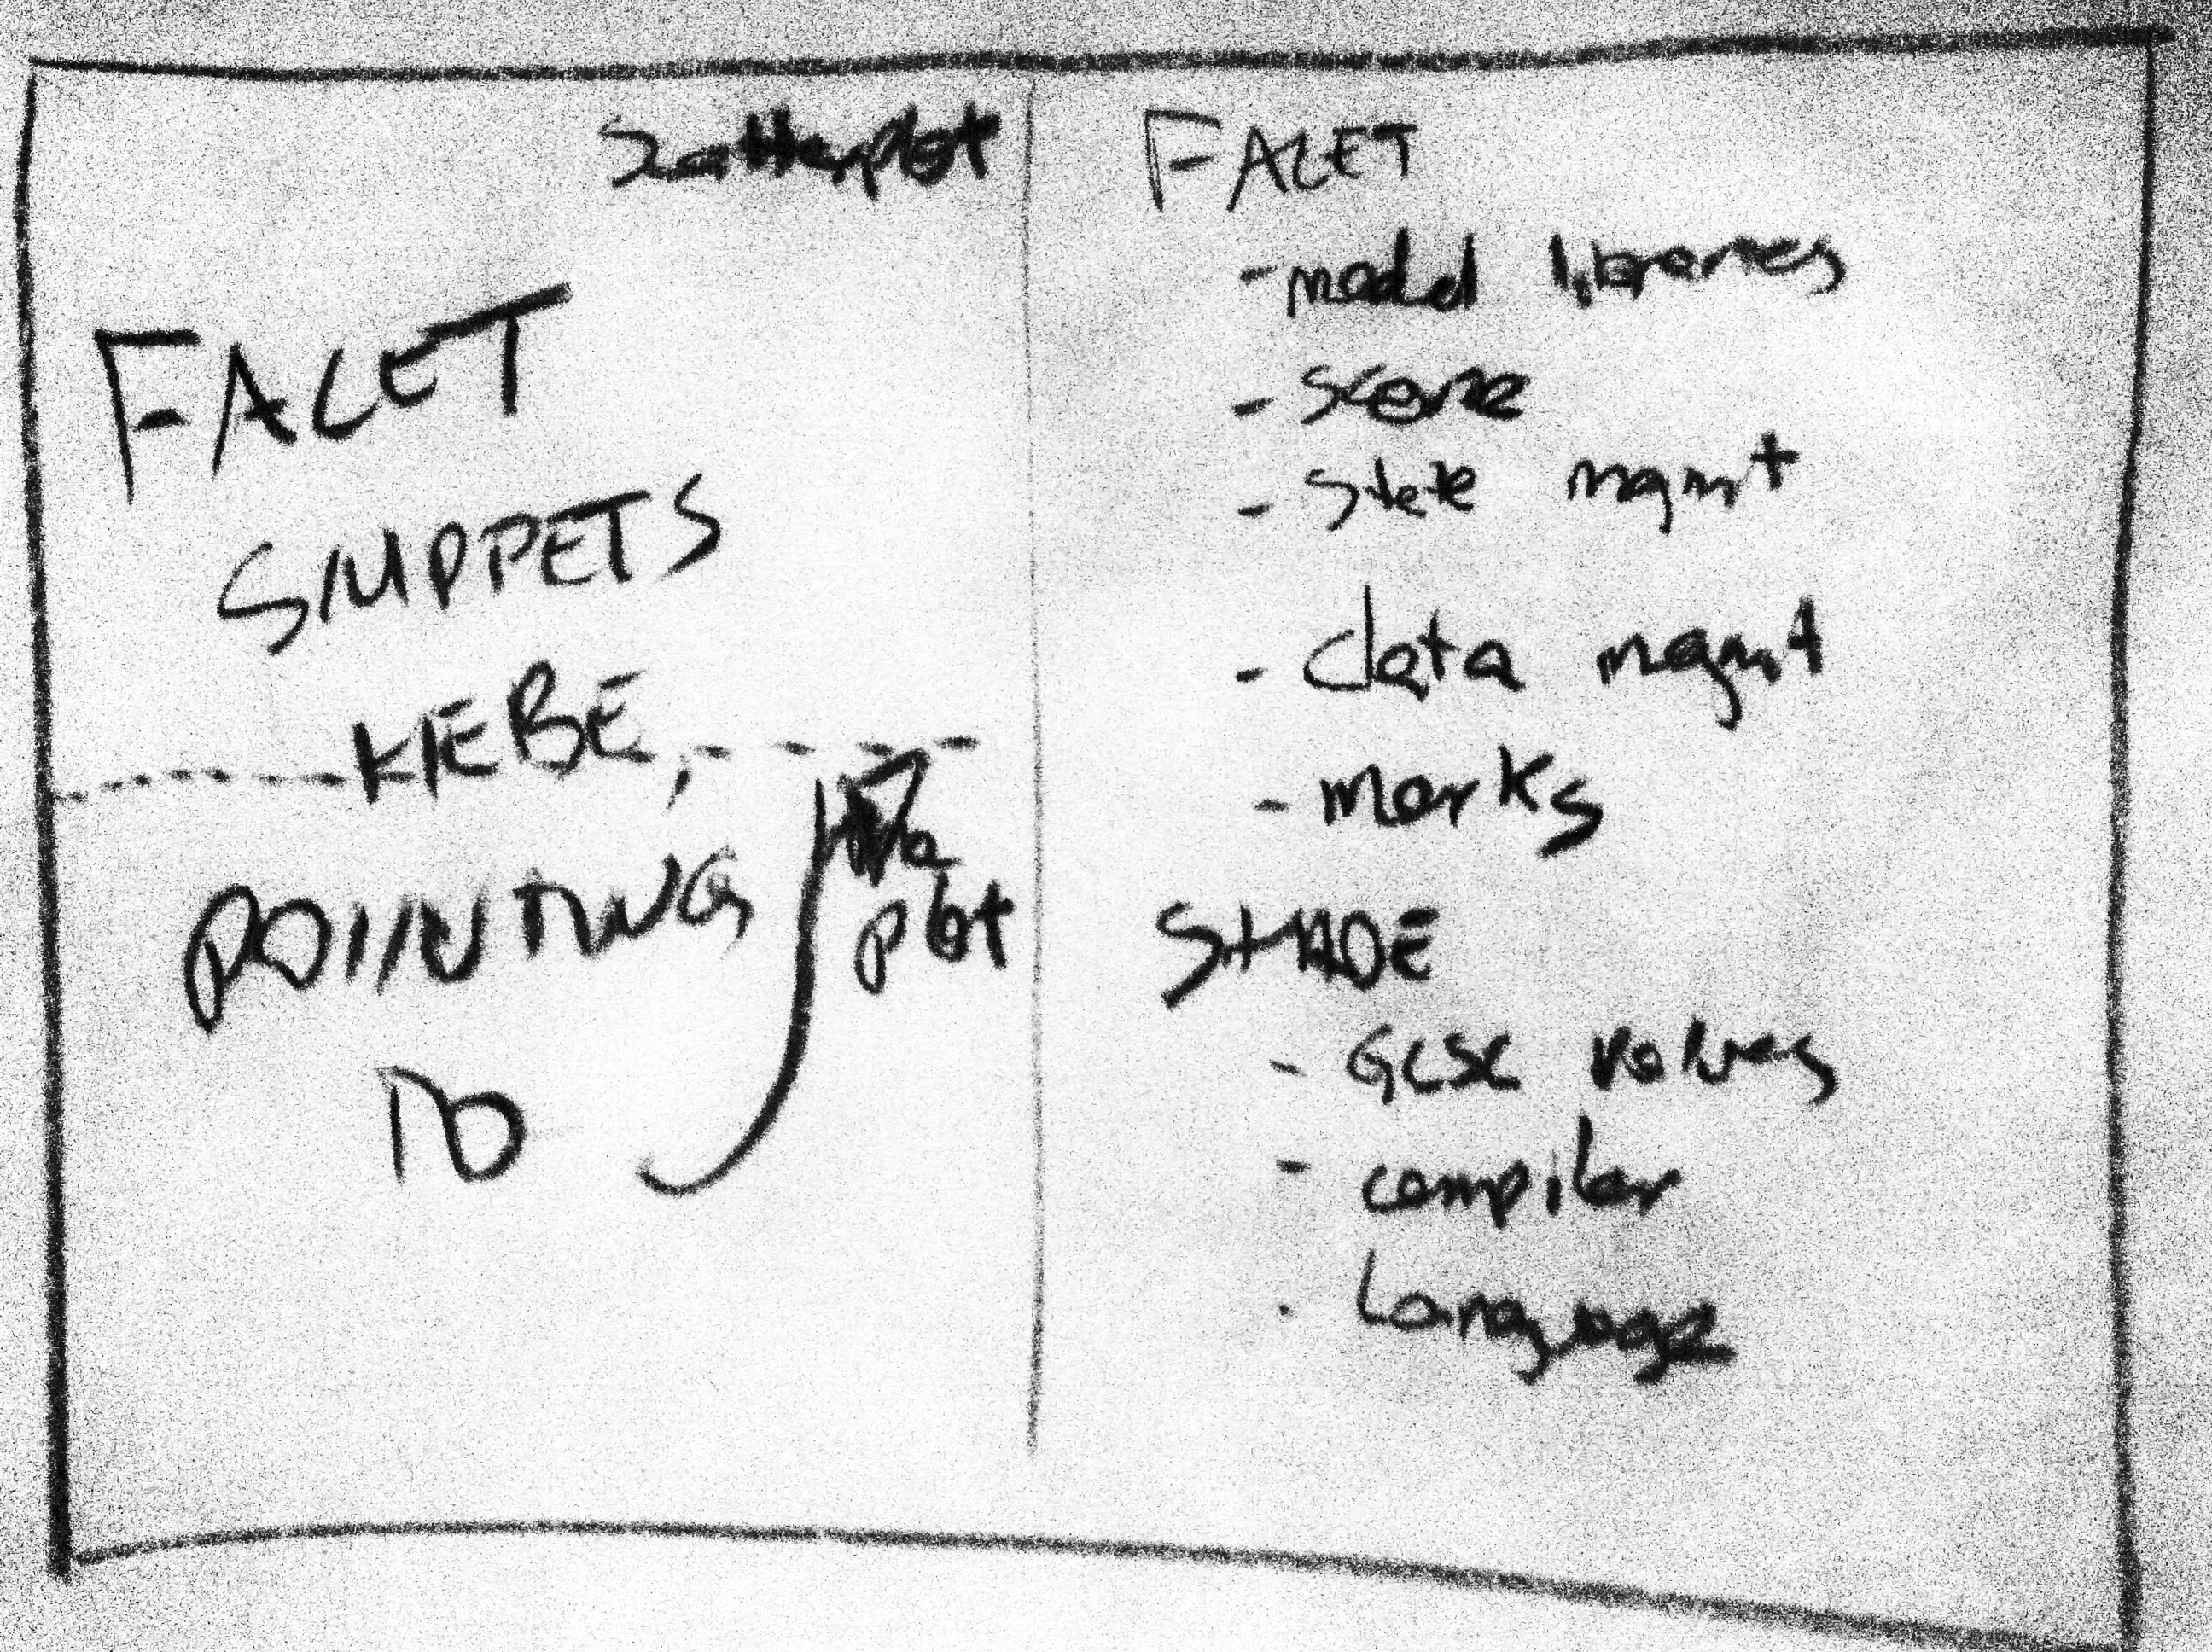
\includegraphics[width=\linewidth]{fig/snippet_overview/overview.jpg}
\caption{Some snippets of Lux code, and their relationship to the
library structure.\label{fig:facetsnippet}}
\end{figure}

Before Lux is described in earnest, let us review an extremely
simple program written in GLSL, WebGL's language for specifying GPU
computations. The first thing to note is that when programming GLSL,
there are in fact two programs one needs to write. The program which
specifies vertex processing is known as the \emph{vertex shader}, and
the program which specifies fragment processing is known as
the \emph{fragment shader} (\emph{fragments} are pixel-sized pieces of
triangles which are given final colors to be rendered on the
screen). The vertex shader mostly computes the position of the vertices,
and the fragment shader, the color of the triangles:

\begin{verbatim}
// Vertex shader
attribute vec4  world_pos, color_in;
uniform   mat4  transform;
varying   vec4  color;
void main()
{
    gl_Position = transform * world_pos;
    color = color_in;
}
// Fragment shader
varying vec4 color;
void main()
{
    gl_FragColor = color;
}
\end{verbatim}

It is important to notice the different types of declarations used for
the different variables. ``Attributes'' denote data which changes
with every vertex, like position and color in the example. Attribute
arrays are advanced in lockstep, so in a model with $n$ vertices, all
attribute arrays must have exactly $n$ entries in memory. ``Uniforms'' are
values which are constant across the entire array of vertices, like the
transformation from world to screen coordinates. ``Varying'' variables
denote values to be interpolated along vertices so they can be
processed by the fragment programs. Note, in addition, that the
fragment shader cannot access \texttt{color\_in} directly: it must go
through a varying variable. This presents a significant reuse problem:
if a user decides to change the data access patterns (which, as we
have argued in Section~\ref{sec:mismatch}, is very likely to happen
across different visualization techniques), shaders which specify
roughly the same operation need to written differently. Worse still,
the WebGL calls to change attribute arrays and uniforms are entirely
different. Creating reusable shader libraries is then very unlikely.

To address this issue, Lux defers the creation of GLSL shaders as
long as possible. Instead, users create and manipulate \Shade
values. \Shade values are Javascript objects which
values in GLSL. For example, \texttt{Shade(5)} is a Javascript object that
denotes the value \texttt{5};
\begin{verbatim}
function f(x, y) {
  return x.mul(y).add(5);
}
\end{verbatim}
\noindent is a Javascript function which takes two \Shade values $x$
and $y$, and returns a new \Shade value denoting $xy + 5$. (the method
syntax is unfortunately inevitable, since Javascript does not support
operator overloading). Lux provides a sizable library of
builtin \Shade functions, which create and manipulate \Shade values
(examples: \texttt{Shade.sin}, \texttt{Shade.cos}, \texttt{Shade.min},
\texttt{Shade.max}, \texttt{Shade.pow}, etc). The entire set of GLSL
built-in functions~\cite{opengles-spec} is available for use as \Shade
functions.

Users build visual primitives by combining \Shade expressions into
larger building blocks. In its lowest-level layer, Lux has two main
data structures: the \emph{model}, and the \emph{batch}. Consider the
following complete (albeit trivial) Lux example:
\begin{verbatim}
gl = Lux.init(canvas);
model = Lux.model({
  type: "triangles",
  elements: 3,
  vertex: [[0,0], [1,0], [1,1]]
});
camera = Shade.Camera.perspective();
triangle = Lux.bake(model, {
  position: camera(model.vertex),
  color: Shade.color("white")
});
Lux.Scene.add(triangle);
\end{verbatim}
The variable \texttt{model} holds a Lux \emph{model}, which says
that the visual primitive will be made out of triangles (other
possibilities include lines and points), and that there are exactly
three vertices (so one total triangle). The variable \texttt{triangle}
holds the result of \texttt{Lux.bake}, known as
a \emph{batch}. \texttt{Lux.bake} combines a model with \Shade
values for the vertex position and color, calls the \Shade compiler to
build the following GLSL program pair:
\begin{verbatim}
// vertex program
attribute vec2 _unique_name_2;
void glsl_name_6 (void) {
  ( gl_Position = 
    (mat4(1.60947, 0.0, 0.0, 0.0, 
          0.0, 2.41421, 0.0, 0.0, 
          0.0, 0.0, -1.00200, -1.0, 
          0.0, 0.0, -0.20020, 0.0) * 
    vec4(_unique_name_2, 0.0, 1.0)) ) ;
}
void main() { glsl_name_6(); }
// fragment program
void glsl_name_1 (void) {
  ( gl_FragColor = vec4(1.0, 1.0, 1.0, 1.0) ) ;
}
void main() {
  glsl_name_1() ;
}
\end{verbatim}
If we were to change the Lux program slightly:
\begin{verbatim}
gl = Lux.init(canvas);
model = Lux.model({
  type: "triangles",
  elements: 3,
  vertex: [[0,0], [1,0], [1,1]],
  color: [color("red"), color("green"), 
          color("blue")], // <-- NEW
});
camera = Shade.Camera.perspective();
triangle = Lux.bake(model, {
  position: camera(model.vertex),
  color: model.color // <-- NEW
});
Lux.Scene.add(triangle);
\end{verbatim}
Lux would then construct a shader with the
appropriate new \emph{attribute} and \emph{varying} bindings:
\begin{verbatim}
// vertex program
attribute vec2 _unique_name_2;
attribute vec4 _unique_name_3; // <-- NEW
varying vec4 _unique_name_4; // <-- NEW
void glsl_name_6 (void) {
  ( gl_Position = 
    (mat4(1.60947, 0.0, 0.0, 0.0, 
          0.0, 2.41421, 0.0, 0.0, 
          0.0, 0.0, -1.00200, -1.0, 
          0.0, 0.0, -0.20020, 0.0) * 
    vec4(_unique_name_2, 0.0, 1.0)) ) ;
}
void glsl_name_8 (void) {
  ( _unique_name_4 = _unique_name_3; );
}
void main() { glsl_name_6(); glsl_name_8(); }
// fragment program
varying vec4 _unique_name_4; // <-- NEW
void glsl_name_1 (void) {
  ( gl_FragColor = _unique_name_4; );
}
void main() {
  glsl_name_1() ;
}
\end{verbatim}

Many users of Lux will never need to \texttt{bake} their own batches
from low-level models, since Lux provides higher-level \emph{marks}
from which to build visualizations (the name ``mark'' comes from the
Protovis concept of the same name~\cite{Bostock:2009:PAG}). Lux
marks take \Shade value parameters which provide data-to-visual
transformations, etc, and create batches that are ready to be added to
the scene. A simple example of a scatterplot is shown in
Figure~\ref{fig:facetsnippet}. We highlight that there is nothing
special about marks as they are written in the Lux: they are simply
convenience layers written on top of lower-level layers. This is an
example of the \emph{composability} advantages of an DSEL approach:
the visual specification can be composed seamlessly from independent
parts.

%% Describe WebGL shortcomings.

%% Uniforms, attributes, varying; all have different APIs and slightly
%% incompatible uses, but they should all be fundamentally
%% interchangeable: they denote \emph{values of a certain type}.

\section{Case Studies and Evaluation\label{sec:evaluation}}

We start this section highlighting some of features of Lux through a
sequence of progressively more complex examples. We then compare the
library performance to current publicly available visualization
libraries. This section is not meant to be a comprehensive guide to
Lux's feature set, but rather a look at the consequences of its
design and impact on how visualization and graphics programs are written.

\subsection{Geographical data on the globe}

Start with a mesh; transform into a sphere; transform to mercator
coordinates; fetch texture; transform lat longs into spherical;

Map different attributes to different visuals. Dot size and color seem
like good ideas.

% Sphere: attribute or shader? Don't know, don't care
\begin{verbatim}
var sphere = function(long_segs, lat_segs)
{
    var uv_mesh = mesh(long_segs, lat_segs);
    var theta = mul(uv_mesh.u, 2 * PI);
    var phi = mul(uv_mesh.v, PI);
    var v = vec(mul(cos(theta), sin(phi)),
                cos(phi),
                mul(sin(theta), sin(phi)));
    return model({ vertex: v,
                   normal: v,
                   elements: uv_mesh.elements,
                   type: uv_mesh.type
                 });
}
\end{verbatim}

The procedure starts from a more basic Lux model (the \emph{mesh}),
which simply encodes a square patch in $[0,1]^2$ tesselated to the
desired detail. It then computes a sphere by transforming the patch
appropriately. \texttt{uv\_mesh.u} and \texttt{uv\_mesh.v} are not
arrays of coordinates, and neither are \texttt{cos(theta)},
\texttt{sin(theta)}, etc: they are shade tree expressions which encode
a value to be computed in a WebGL shader. This has important
consequences. For example, if any of the sphere fields end up being
used in expressions that must be computed by the fragment shader (for
example, a normal could be used in cube mapping), Lux will
automatically split the necessary computations between WebGL
\emph{attributes} and WebGL \emph{varying}s, the former only being
allowed in vertex shaders, and the latter only in fragment shaders. By
relieving the user from making this decision, Lux allows increased
code reuse and expressivity.

\subsection{Custom shapes and picking}

% Picking wedges: automatically creating new shaders from old.
Expressing WebGL shader computations directly in Lux objects has
another substantial advantage: Lux can manipulate these expressions
programatically, and automatically create derived expressions. A
particularly useful example comes from Lux's implementation of
picking functionality (that is, determining which object lies under
the cursor). Lux uses a popular approach to OpenGL picking, which is
to render the exact same scene to an offscreen buffer, only replacing
final fragment colors with \emph{object ids}. The pixel under the
cursor is then read back from the GPU into main memory.
%
Lux allows
users to write arbitrary shading expressions, which include
statements that \emph{discard} some fragments. Rendering complex shapes through appropriate use of the
discard statement is a popular way to achieve resolution
independence and pixel precision without tesselation, as for example
has been shown by Loop and Blinn for Bezier
curves~\cite{Loop:2005:RIC}.
%
To ensure that the picking buffer is drawn exactly in the
same way as the regular screen, it is necessary to write custom
paired shaders: one picking shader for every rendering
shader. Requiring these to be written manually is cumbersome,
inelegant, and error-prone. Lux, on the other hand,
\emph{automatically} calculates the picking shader from the rendering
shader. Any model with a \texttt{id} field in its appearance can be
drawn in both rendering and picking mode. 

\subsection{Performance}

\begin{figure*}
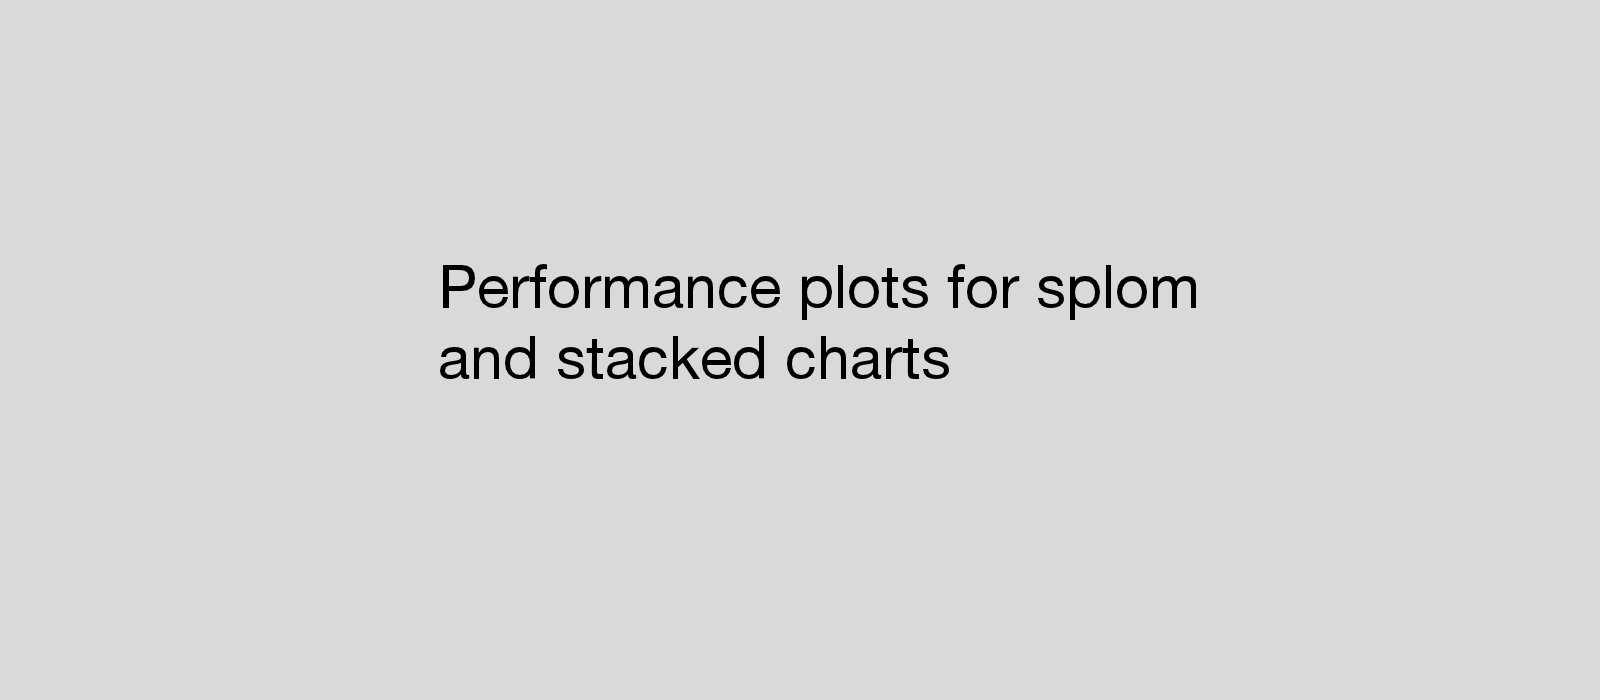
\includegraphics[width=\linewidth]{fig/performance/performance.jpg}
\caption{Comparing the performance of Lux to D3 and Protovis on two
standard benchmarks: a scatterplot matrix and a stacked graph}
\end{figure*}

Scale: Plot every zip7 centroid on top of an openstreetmap globe?
Rebuild zipscribble?

NEED TO SHOW PROCESSING.JS, PROTOVIS AND D3 AT THE VERY LEAST HERE.

WHAT ABOUT TRADITIONAL scivis?

volume rendering, streamlines? Those are both fairly challenging
because of the integrals and ODEs. Volume rendering is a little easier
because the end result is a single value per integral, while
streamlining requires access the full function after we integrate the
differential equation. How I wish I had geometry shaders...

Loops, geometry shaders.

SO, how do we reimplement geometry shaders in Lux?

\section{Discussion\label{sec:discussion}}

Animation, cost to recompile shaders, ease of programming.

Having a model of GLSL values in Javascript is important for
testing. Mention that this was used during the development of Lux
itself.


\section{Conclusion}

This paper argues that careful API design can have a large impact in
how visualization and 3D graphics software is written on the Web, and
contributes Lux as an example of how to address some of these
shortcomings.

We believe we have but scratched the surface of this area.
% So what do we do now with Lux?

\bibliographystyle{eg-alpha}
\bibliography{paper}

\end{document}
